\section{Auswertung}

Bei den Messungen wurden folgende Komponenten verwendet, die bei den anschließenden
Berechnungen als fehlerfrei betrachtet werden:

\begin{align}
  L        &= 32.51              \, \su{mH}       \\
  C        &= 8.01 \cdot 10^{-10}  \, \su{F}       \\
  C\ua{Sp} &= 3.7 \cdot 10^{-10}    \, \su{F}       \\
  R        &= 48                   \, \su{\Omega}
\end{align}

Bei dem $C\ua{Sp}$ handelt es sich dabei um die Kapazität, die jede Spule besitzt
und die bei den Rechnungen ebenfalls beachtet werden muss.

\subsection{Justierung der Schwingkreise}

Vor den Messungen wurden die beiden Schwingkreise so justiert, dass sie die
selbe Resonanzfrequenz besitzen. Bei der Messung ergab sich als Resonanzfrequenz
für den linken Schwingkreis folgender Wert:

\begin{equation}
  \nu^+ = 31.10 \su{kHz}.
\end{equation}

Mithilfe der Formel \eqref{eqn:nu+} kann der Wert für $\nu_t^{+}$ ebenfalls bestimmt werden,
sodass sich für die beiden Frequenzen eine Abweichung von ca. 2 \% ergibt. Der
berechnete Wert für $\nu_t^{+}$ kann Tabelle \ref{tab:Messungb} entnommen werden.

\subsection{Bestimmung des Verhältnisses zwischen Schwingung und Schwebung}


Mithilfe der Formeln \eqref{eqn:nu+} und \eqref{eqn:nu-} werden ebenfalls die theoretischen Frequenzen
$\nu_t^{+}$ und $\nu_t^{-}$ aus den oben angegebenen Bauteilen bestimmt und mit
folgender Formel das Verhältniss bestimmt:

\begin{equation}
  n_t = \frac{\nu_t^{+} + \nu_t^{-}}{2(\nu_t^{-} - \nu_t^{+})}.
\end{equation}

In Tabelle \ref{tab:Messunga} sind die bestimmten Werte sowie die Abweichungen von
experimentell bestimmten Werten zu den theoretisch berechneten Werten zu sehen.
Die Abweichung berechnet sich dabei nach folgender Formel:

\begin{equation}
  a = \frac{\increment n}{n} = \frac{|n-n\ua{t}|}{n}.
  \label{eqn:Abweichungen}
\end{equation}

\begin{table}
  \centering
  \begin{tabular}{c | c | c | c | c | c | c | c}
  \toprule $C\ua{k}$ in $\su{nF}$ & $\sigma\ua{C\ua{k}}$ in $\su{nF}$ & $n$
           & $\nu_t^{+}$ in $\su{kHz}$ & $\nu_t^{-}$ in $\su{kHz}$
           & $\sigma\ua{\nu_t^{-}}$ in $\su{kHz}$ & $n\ua{t}$ & $a$ in $\su{\%}$ \\
  \midrule
  9.99 & 0.03 & 14 & 30.492 & 32.730 & 0.006 & 14.1 & 0.8 \\
  8.00 & 0.02 & 12 & 30.492 & 33.259 & 0.008 & 11.5 & 4.0 \\
  6.47 & 0.02 & 10 & 30.492 & 33.87 & 0.01 & 9.5  & 5.0 \\
  5.02 & 0.02 & 8  & 30.492 & 34.78 & 0.01 & 7.6  & 5.0 \\
  4.00 & 0.01 & 6  & 30.492 & 35.77 & 0.01 & 6.3  & 5.0 \\
  3.00 & 0.009 & 5  & 30.492 & 37.33 & 0.02 & 5    & 0.8 \\
  2.03 & 0.006 & 4  & 30.492 & 40.09 & 0.03 & 3.7  & 8.0 \\
  1.01 & 0.003 &    & 30.492 & 47.40 & 0.04 & 2.3  &     \\
  \bottomrule
  \end{tabular}
 \caption{Bestimmte Werte für die Fundamentalfrequenzen und Vergleich der
          gemessenen und berechneten Verhältnisse}
 \label{tab:Messunga}
\end{table}

Da bei dem Bestimmen der Anzahl an Maxima der Schwingung in einem Schwebungsbauch
vor allem an den äußeren Rändern die Maxima nicht klar erkennbar sind, wird bei den
gemessenen Werten ein Fehler von $\pm 1$ angegeben.

Für die letzte Kapazitätseinstellung konnte die Anzahl an Maxima nicht eindeutig
bestimmt werden, deswegen kann hier kein Vergleich mit den theoretischen Werten
erfolgen.

In der Tabelle ist jedoch deutlich zu sehen, dass mit sinkender Kopplungskapazität
auch das Verhältnis der Schwingungs- und Schwebungsfrequenz immer geringer wird.

Die angegebenen Fehler berechnen sich dabei mit der Gaußschen Fehlerfortpflanzung
und berechnen sich wie folgt:

Da bei allen Bauteilen, außer dem Kopplungskondensator, eine Fehlerfreiheit
vorausgesetzt wurde, ergibt sich aufgrund der in Formel \eqref{eqn:I(w^-)} erkenntlichen fehlenden
Abhängigkeit für $\nu_t^{+}$ kein Fehler und für $\nu_t^{-}$ folgende Fehlerformel:

\begin{align}
  \increment \nu_t^{-} &= \sqrt{(\partial_{C\ua{k}} \nu_t^{-} \cdot \increment C\ua{k})^2} \\
                       &= -2\pi\left[ L^3 \left[ \left( \frac{1}{C} + \frac{2}{C\ua{k}}\right)^{-1}
                          + C\ua{Sp} \right]^3 \right]^{-\frac{1}{2}} \frac{L}{\left( \frac{C\ua{k}}{C} + 2 \right)^2} \cdot \increment C\ua{k}
\end{align}

\subsection{Bestimmung der Fundamentalfrequenzen mithilfe einer erzwungenen Schwingung}

Mithilfe einer erzwungenen Schwingung und verschiedenen Einstellungen des
Kopplungskondensators können die beiden Fundamentalfrequenzen experimentell
bestimmt werden. In Tabelle \ref{tab:Messungb} sind die gemessenen Frequenzen sowie deren
Abweichungen zu den theoretisch bestimmten Werten zu sehen. Es handelt sich dabei
um die in Tabelle \ref{tab:Messunga} angegebenen Werte.

Die Abweichungen werden dabei analog zu Formel \eqref{eqn:Abweichungen} bestimmt.

\begin{table}
  \centering
  \begin{tabular}{ c | c | c | c | c }
    \toprule $C\ua{k}$ in $\su{nF}$
           & $\nu_{+}$ in $\su{kHz}$ & $a\ua{\nu_{+}}$ in $\su{\%}$
           & $\nu_{-}$ in $\su{kHz}$ & $a\ua{\nu_{-}}$ in $\su{\%}$ \\
    \midrule
    9.99 & 30.77 & 0.9 & 33.16 & 1.3 \\
    8.00 & 30.79 & 1.0 & 33.66 & 1.2 \\
    6.47 & 30.80 & 1.0 & 34.25 & 1.1 \\
    5.02 & 30.81 & 1.0 & 35.12 & 1.0 \\
    4.00 & 30.82 & 1.1 & 36.08 & 0.9 \\
    3.00 & 30.83 & 1.1 & 37.60 & 0.8 \\
    2.03 & 30.84 & 1.1 & 40.28 & 0.5 \\
    1.01 & 30.85 & 1.2 & 47.33 & 0.2 \\
    \bottomrule
  \end{tabular}
  \caption{Gemessene Fundamentalfrequenzen und die Abweichungen zu den theoretisch
           berechneten Werten}
  \label{tab:Messungb}
\end{table}

Die bestimmten Fundamentalfrequenzen und die Theoriewerte sind in Abbildung \ref{fig:Messungb}
noch einmal grafisch dargestellt. Wie erwartet ist der Wer für $\nu_{+}$ nahezu
konstant und der wert von $\nu_{-}$ zeigt einen Abfall. Beide
Werte liegen dabei nahe an den Theoriewerten.

\begin{figure}
 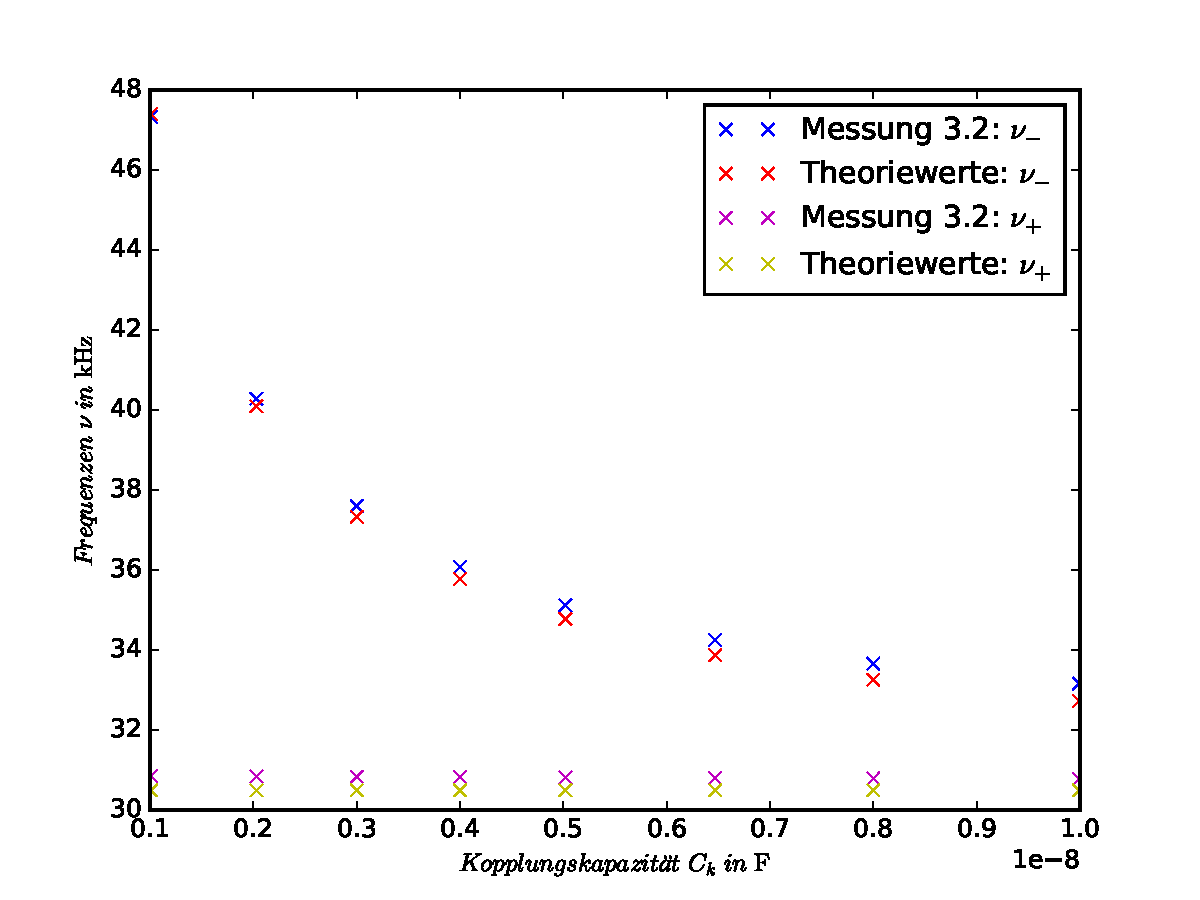
\includegraphics[width=\textwidth]{Messungb_Plot1.pdf}
 \caption{Vergleich der in Messung 3.2 bestimmten Werte mit den Theoriewerten}
 \label{fig:Messungb}
\end{figure}

\newpage

\subsection{Bestimmung der Fundamentalfrequenzen mittels einenes Sweeps}

In dem letzen Teil der Messung wurden mithilfe eines Sweeps erneut die beiden
Fundamentalfrequenzen bestimmt. Dazu wurden sowohl Startwert, Endwert sowie auch
Zeitspanne des Sweeps eingestellt. Um die Messungen zu vereinfachen wurden der
Startwert $\nu\ua{S}$ und Endwert $\nu\ua{E}$ jedes Mal so angepasst, dass der
Startwert mit den vorher bestimmten Werten für $\nu_t^{+}$ übereinstimmt. Lediglich
die Dauer des Sweeps wurde konstant bei $t\ua{S}$ = 2 Sekunden gelassen.

Am Oszilloskop wurde dann bei der Messung die Zeitspanne zwischen dem ersten
Spannungsmaximum und dem zweiten Spannungsmaximum $t\ua{D}$ gemessen. Mit folgender
Formel kann dann der Frequenzwert für $\nu_{-}$ bestimmt werden:

\begin{equation}
  \nu_{-} = \nu\ua{S} + \frac{t\ua{D}}{t\ua{S}} \cdot ( \nu\ua{E} - \nu\ua{S}).
\end{equation}

In Tabelle \ref{tab:Messungc} sind die verschiedenen bestimmten Werte eingetragen, sowie für
die Fundamentalfrequenz  $\nu_{-}$ die Abweichungen zu den theoretischen Werten.

\begin{table}
  \centering
  \begin{tabular}{ c | c | c | c | c | c | c }
    \toprule $C\ua{k}$ in $\su{nF}$
           & $\nu_{+} \, (\nu\ua{S})$ in $\su{kHz}$ & $\nu\ua{E}$ in $\su{kHz}$
           & $t\ua{D}$ in $\su{s}$ & $\nu_{-}$ in $\su{kHz}$
           & $\increment \nu_{-}$ in $\su{kHz}$ & $a\ua{\nu_{-}}$ in $\su{\%}$ \\
    \midrule
    9.99 & 30.77 & 40.00 & 0.500 & 33.078 & 0.605 & 1.0 \\
    8.00 & 30.79 & 40.00 & 0.600 & 33.533 & 0.479 & 0.9 \\
    6.47 & 30.80 & 40.00 & 0.740 & 34.204 & 0.229 & 1.0 \\
    5.02 & 30.81 & 40.00 & 0.925 & 35.060 & 0.230 & 0.8 \\
    4.00 & 30.82 & 40.00 & 1.125 & 35.984 & 0.230 & 0.6 \\
    3.00 & 30.83 & 40.00 & 1.475 & 37.593 & 0.230 & 0.7 \\
    2.03 & 30.84 & 50.00 & 1.000 & 40.420 & 0.230 & 0.8 \\
    1.01 & 30.85 & 55.05 & 1.360 & 47.306 & 0.231 & 0.2 \\
    \bottomrule
  \end{tabular}
  \caption{Mithilfe der Sweep-Methode bestimmte Werte für die Fundamentalfrequenzen
           und die Abweichungen zu den theoretisch bestimmten Werten}
  \label{tab:Messungc}
\end{table}

Da das Ablesen auf dem Oszilloskop nicht genau ist, wird für die gemessenen
Zeiten ein Fehler von $\pm$ 0.05 Sekunden berücksichtigt, welcher in der Tabelle
\ref{tab:Messungc} nicht mit angegeben ist.

Auch hier wurden die Fehler mit der Gaußschen Fehlerfortpflanzung berechnet:

\begin{align}
  \increment \nu_{-} &= \sqrt{\left(\partial_{t\ua{D}} \nu_{-} \cdot \increment t\ua{D}\right)^2} \\
                     &= \frac{1}{t\ua{S}}\cdot ( \nu\ua{E} - \nu\ua{S}) \cdot \increment t\ua{D} .
\end{align}

\begin{figure}
 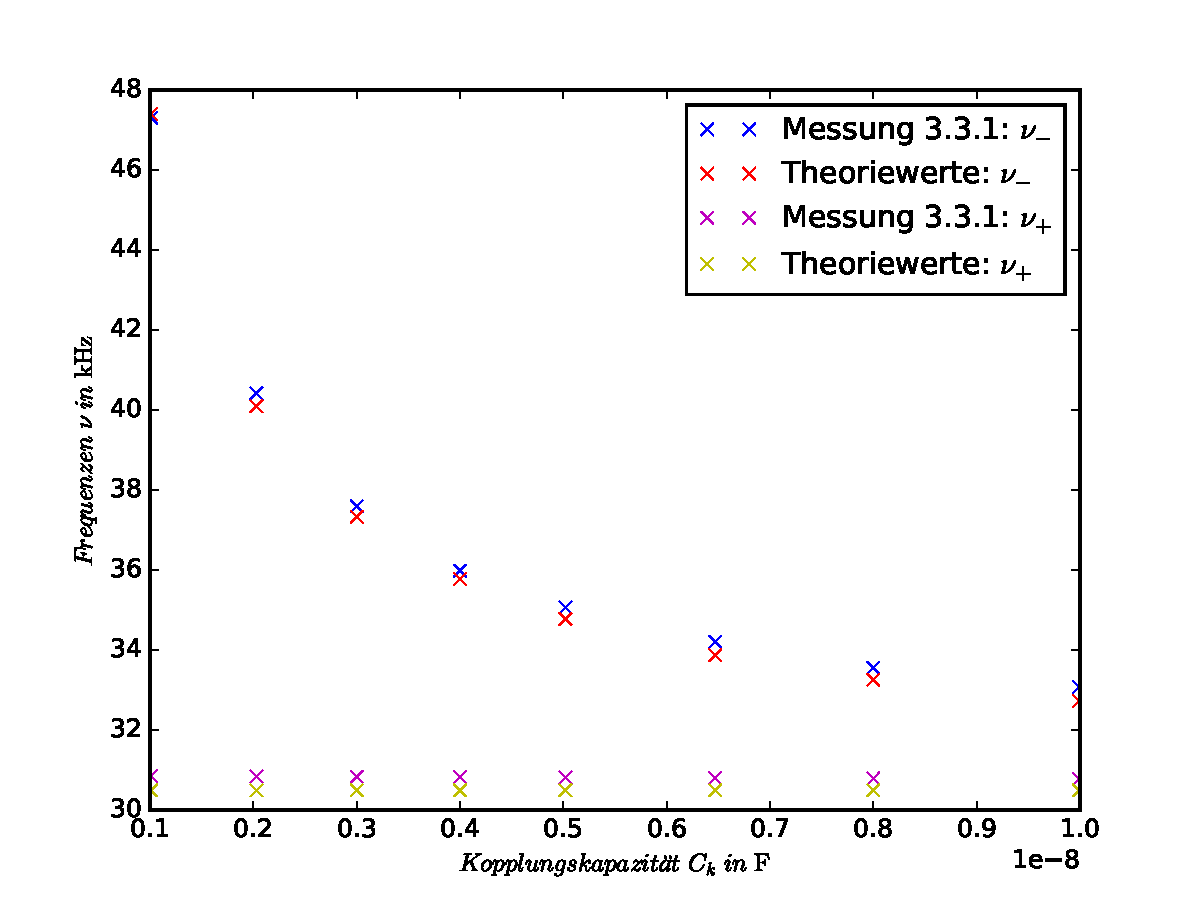
\includegraphics[width=\textwidth]{Messungc_Plot1.pdf}
 \caption{Vergleich der in Messung 3.3.1 bestimmten Werte mit den Theoriewerten}
 \label{fig:Messungc}
\end{figure}

Auch hier sind die berechneten Frequenzen sowie die Theoriewerte noch einmal grafisch
in Abbildung \ref{fig:Messungc} dargestellt. Wie schon bei der vorherigen Messung
kann man einen konstanten Wert für $\nu_{+}$ sowie einen
Abfall bei $\nu_{-}$ beobachten, wobei erneut die Werte nicht bedeutend von den
Theoriewerten abweichen, wie auch schon in der Tabelle \ref{tab:Messungc}
sichtbar.

\section{Diskussion}

In diesem Abschnitt geht es darum, die gewonnen Messdaten hinsichtlich der
Messqualität zu bewerten.

In der ersten Messung des Versuches wurde das Verhältnis von Schwebungs- und
Schwingungsfrequenz bestimmt. In Tabelle \ref{tab:Messunga} ist erkennbar, dass
die Abweichungen der experimentell bestimmten Werte zu den Theoriewerten relativ
schwankend sind und von einem Fehler von 0.8 $\%$ $(C\ua{k} = 3.00 \, \su{nF})$ bis
zu einem Fehler von 8.0 $\%$ $(C\ua{k} = 2.03 \, \su{nF})$ reichen.

Wie in den beiden Abbildungen \ref{fig:Messungb} und \ref{fig:Messungc} erkennbar
ist, weichen die experimentell bestimmten Werte in den Messung 3.2 und 3.3.1
nur minimal von den Theoriewerten
ab. Die Tabellen \ref{tab:Messungb} und \ref{tab:Messungc} zeigen beide, dass die
Abweichungen der Werte von $\nu_{+}$ und $\nu_{-}$ lediglich im Bereich von ca.
einem Prozent liegen. Zudem sind die Theoriewerte von $\nu_t^{-}$ alle im Bereich
der in Messung 3.3.1 bestimmten Fehler für $\nu_{-}$.

Die Abweichungen der Werte können jedoch auf getroffene Annahmen zurückgeführt
werden. Zum einem werden die verwendeten Bauteile bei dem Versuch, mit Ausnahme
des Kopplungskondensators, als fehlerfrei angenommen.
Die bei Messung 3.2 verwendete Methode ist zudem ziemlich ungenau, was sich auch
darin widerspiegelt, dass für die Einstellung $C\ua{k} = 1.01 \su{nF}$ kein
Wert für die Anzahl an Maxima bestimmt werden konnte. Vor allem die Differenzierung
der Maxima an den äußeren Rändern der Schwebung stellte sich als kompliziert
heraus. Des Weiteren wird die abgelesene Frequenz bei dem Generator ebenfalls als
fehlerfrei angenommen.

Zusammenfassend ist jedoch erkenntlich, dass sowohl die in Messung 3.3.1 als auch die
in Messung 3.3.1 verwendeten Messmethoden geeignet sind, um die beiden Fundamentalfrequenzen
bis auf eine Abweichung von ca. 1 $\%$ genau zu bestimmen. Lediglich die bei Messung 3.2 verwendete Methode
scheint ziemlich ungenau zu sein und ist daher für die genauere Bestimmung des
Frequenzverhältnisses nicht zu empfehlen.
